% Copyright 2010 by Stefano Maggiolo and Nicola Pagani

\documentclass{amsart}

\usepackage[english]{babel}
\usepackage{amssymb}
\usepackage{hyperref}
\usepackage{tikz}
\usepackage{booktabs}
\usepackage{multirow}
\usepackage{mathtools}

\newcommand{\arXiv}[1]{\href{http://arxiv.org/abs/#1}{arXiv:#1}}

\theoremstyle{plain}
\newtheorem{theorem}{Theorem}[section]
\newtheorem{proposition}[theorem]{Proposition}
\newtheorem{corollary}[theorem]{Corollary}
\newtheorem{lemma}[theorem]{Lemma}
\theoremstyle{definition}
\newtheorem{remark}[theorem]{Remark}
\newtheorem{example}[theorem]{Example}
\newtheorem{definition}[theorem]{Definition}
\newtheorem{notation}[theorem]{Notation}


\DeclareMathOperator{\bN}{\mathbb{N}}
\DeclareMathOperator{\mult}{mult}
\DeclareMathOperator{\MAX}{max}
%\DeclareMathOperator{\min}{min}

\newcommand{\graph}{\mathcal{G}}
\newcommand{\abs}[1]{\left|#1\right|}
\newcommand{\ubar}[1]{\underline{#1}}
\newcommand{\obar}[1]{\overline{#1}}
\newcommand{\psm}[1]{\left(\begin{smallmatrix}#1\end{smallmatrix}\right)}

\title{Generating stable modular graphs}
\author{Stefano Maggiolo}
\author{Nicola Pagani}
\date{\today}

\begin{document}

\begin{abstract}
  We present the program \texttt{strata}, whose source files are
  available at \href{http://people.sissa.it/~maggiolo/strata/}
  {\texttt{http://people.sissa.it/\~{}maggiolo/strata/}}. Given two
  natural numbers $g$ and $n$ satisfying $2g+n-2>0$, the program
  generates all genus $g$ stable graphs with $n$ half-edges. Each such
  graph determines the topological type of a nodal stable curve of
  arithmetic genus $g$ with $n$ marked points. Our motivation comes
  from the fact that the boundary of the moduli space of stable genus
  $g$, $n$-pointed curves can be stratified by taking loci of curves
  of a fixed topological type.
\end{abstract}

\maketitle
\setcounter{tocdepth}{1}
\tableofcontents


\section{Introduction}
Moduli spaces of smooth algebraic curves have been defined and then
compactified in algebraic geometry by Deligne and Mumford in their
seminal paper~\cite{delignemumford}. The points in the boundary
correspond to nodal curves with finite automorphism group. These
curves are called \emph{stable curves}. The topology of one such curve
is encoded in a combinatorial object, called \emph{stable graph}. The
boundary of the moduli space admits a topological stratification,
whose elements are curves with fixed topology.

The combinatorics of the stable graphs have been investigated in
several papers in algebraic geometry, for many different purposes (see
for instance~\cite{modularoperads,opstall,opstall2,stephanie2}). Our
aim with this program is to provide an useful and effective tool to
generate all the stable graphs of genus $g$ with $n$ marked points up
to isomorphism, for low values of $g$ and $n$.

We construct an algorithm to generate all the stable, $n-$pointed
graphs of genus $g$. Then we use the library nauty~(\cite{nauty}) to
eliminate isomorphic graphs from the list of graphs thus
created. Since to check that two stable graphs are isomorphic is
computationally onerous, we try to generate a low number of stable
graphs, provided that we want at least one for every equivalence
class. The algorithm successively calls recursive functions to build
the vectors of genera, marked points, and the adjacency matrix. Then
it checks the stability condition and the condition on the total genus
as early as possible, in order to minimize the time spent on the
branches of the recursion that do not lead to stable graphs. Our
program works effectively with a bound on the maximal number of
vertices: $2g-2+n<13$.

Programs for enumerative computations on
$\overline{\mathcal{M}}_{g,n}$ have been implemented in both Maple and
Macaulay2~(\cite{faber,stephanie1,smith}). Our program can be used,
for example, to improve the results of~\cite[Section 5]{stephanie2},
or to prove simple results on the combinatorics of stable curves with
low genus (cfr.~\cite{busonero}, for example Corollary~5.3).



\section{What to generate}

From now on, we fix two natural numbers $G$ and $N$ such that $2
G-2+N>0$.  For every $K \in \bN^+$, we define $\ubar{K} = \{0, \dots,
K-1\}$. Let $\Sigma_K$ be the symmetric group on the set $\ubar{K}$.

\begin{definition}
  \mbox{}
  \begin{itemize}
  \item An \emph{undirected multigraph\/} $\graph$ is a couple $(V,
    E)$ with $V$ a finite set of \emph{vertices\/} and $E$ a finite
    multiset of \emph{edges\/} with elements in $V \times V/\Sigma_2$.
  \item The multiplicity of $(v, w)$ in $E$ is denoted by $\mult(v,
    w)$.
  \item The \emph{total multiplicity\/} of $\graph$, or its
    \emph{number of edges}, is $\abs{E}$: the cardinality of $E$ as a
    multiset.
  \item The \emph{degree\/} of a vertex $v$ is $\deg v \coloneqq 2
    \mult(v, v) + \sum_{w \neq v} \mult(v, w)$.
  \item A \emph{colored undirected multigraph\/} is a multigraph with
    some additional data attached to each vertex.
  \end{itemize}
\end{definition}

\begin{definition}\label{def:stable graph}
  A \emph{stable graph\/} of type $(G, N)$ is a colored undirected
  multigraph $\graph = (V, E)$, subject to the following conditions.
  \begin{enumerate}
  \item The color of a vertex $v$ is given by a pair of natural
    numbers $(g_v, n_v)$.
  \item \label{it:condition connected} $\graph$ is connected.
  \item \label{it:condition genus} Its \emph{total genus}, defined as
    $\sum_{v \in V} g_v + \abs{E} - (\abs{V} - 1)$, equals $G$.
  \item Its \emph{total number of marked points}, defined as $\sum_{v
      \in V} n_v$, equals $N$.
  \item \label{it:condition stability} Stability condition: $\deg v +
    n_v \geq 3$ for every vertex $v$ with $g_v = 0$ (in other words,
    $v$ must have at least $3$ \emph{half edges\/}).
  \end{enumerate}
\end{definition}

Two stable graphs $\graph = (V, E, g, n)$ and $\graph^\prime =
(V^\prime, E^\prime, g^\prime, n^\prime)$ are \emph{isomorphic\/} if
there is a bijection $f\colon V \to V^\prime$ such that:
\begin{itemize}
\item $\mult(v, w) = \mult(f(v), f(w))$ for every $v, w \in V$;
\item $g_v = g^\prime_{f(v)}$ and $n_v = n^\prime_{f(v)}$ for every $v
  \in V$.
\end{itemize}
Our task is to generate one stable graph for each isomorphism class.

\begin{remark}
  Note that from the definition just given, we are working with an
  unordered set of marked points.
\end{remark}



\section{How the program generates graphs}

Let us introduce the notation we use in the program.

\begin{notation}\label{not:gnla}
  The set of vertices $V$ will always be $\ubar{K}$, so that vertices
  will be identified with natural numbers $i, j, \dots$. The
  multiplicity of the edge between $i$ and $j$ will be denoted by
  $a_{i,j}$: the symmetric matrix $a$ is called the \emph{adjacency
    matrix} of the stable graph. For convenience, we will denote $l_i
  = a_{i,i}$: it is the vector whose elements are the loops at the
  vertex $i$. For simplicity, we will consider $g_i$, $n_i$, $l_i$,
  $a_{i,j}$ to be defined also for $i$ or $j$ outside $\ubar{K}$, in
  which case their value is always assumed to be $0$.
\end{notation}

\begin{remark}
  In the following, we assume $\abs{V} > 1$ in order not to deal with
  special cases. There are trivially $G+1$ stable graphs of type $(G,
  N)$ with one vertex, depending on the number of self intersection of
  the single irreducible component.
\end{remark}

The program uses recursive functions to generate the data that
constitute a stable graph. In order, it generates the numbers $g_i$,
then the numbers $n_i$, $l_i$ (the diagonal part of the matrix $a$),
and finally, row by row, a symmetric matrix representing $a$.

The program follows two principles: the first is to generate the
smallest possible number of couples of isomorphic stable graphs, the
second is to check the conditions of Definition~\ref{def:stable graph}
as early as possible, to minimize the time spent in branches that do
not lead to stable graphs.

To take into account the second principle, we will deduce from the
conditions of Definition~\ref{def:stable graph} some other necessary
conditions that can be checked before the graph is defined in its
entirety. For the first principle, we generalize the following idea:
to generate a vector for every class of vectors of length $K$ modulo
permutations, the simplest way is to generate vectors whose entries
are increasing.

Therefore, the program fills the data in the order
\begin{align*}
  & g_0, \dots, g_{K-1}, \\
  & \qquad \qquad n_0, \dots, n_{K-1}, \\
  & \qquad \qquad \qquad \qquad l_0, \dots, l_{K-1}, \\
  & \qquad \qquad \qquad \qquad \qquad \qquad a_{0,1}, \dots, a_{0,
    K-1}, a_{1, 2}, \dots, a_{1, K-1}, \dots, a_{K-2, K-1}\text{.}
\end{align*}
It fills each of these positions with an integer in a specific range
that we are going to describe in Section~\ref{sec:ranges}. For each of
these attempts, it recursively continues to fill the data until
everything is fixed and the graph is checked to be a stable graph and
not isomorphic to a graph already generated.

% TODO explain better that division is a way to enforce lexicographic
% order on g,n,l,a (scanned horizontally and vertically)
The main ingredient to decide the lower endpoint is the concept of
\emph{division\/} before an index $i$. Basically, having a division
before $i$ means that within the data we have already decided, we have
that a value relative to the index $i$ is strictly bigger than a value
relative to the index $i-1$. Hence, if we have a division before $i$,
we allow the data relative to the index $i$ to start from $0$;
otherwise, it can only start from the value assigned to the index
$i-1$ (i.e., the datum we are deciding must be non decreasing at the
index $i$).

\begin{notation}
  We will denote the endpoints of the range of values that the program
  tries to assign to $g_i$ as $g_i^{\min}$ and $g_i^{\MAX}$;
  \emph{mutatis mutandis\/} for the other data.
\end{notation}

\begin{remark}
  We choose the ranges for the data $g$, $n$, and $l$, in such a way
  that for any data $(g, n, l)$ the program generates, there is at
  least one choice for the matrix $a$ that gives a stable graph.

  % TODO: fix this
  This is so because the endpoints for the ranges are computed
  thinking of the worst possible stable graph (that is, the one with
  the least number of half edges, to stabilize genus $0$ vertices, and
  the least number of edges, to connect the graph). Hence, at least
  this worst case is stable and with those data.
\end{remark}



\section{Description of the ranges}\label{sec:ranges}

\begin{notation}
  At any time during the algorithm, we let $e^{\MAX}$ be the maximum
  number of edges that could be placed after that time, and $c$ be the
  number of couples of (different) vertices already connected by an
  edge. We let $p_1$ be the number of vertices $i$ to which the
  algorithm has assigned $g_i = 0$;
\end{notation}

\begin{notation}
  When deciding $g$, $n$, or $l$, we let $\tilde{n}_i$ be the minimum
  between $2$ and the number of half edges already assigned to the
  $i$-th vertex. This is justified by the fact that we know that at
  least one half edge will be assigned to the $i$-th vertex to connect
  it to the rest of the graph. Hence, whenever $g_i = 0$,
  $\tilde{n}_i$ represent the number of \emph{stabilizing\/} half
  edges, in the sense that they are not useless for the aim of
  stabilizing the curve. We define also
  \begin{align*}
    N_i &\coloneqq \sum_{\substack{j < i\\g_j = 0}} n_j\,\text{,} &
    \tilde{N} &\coloneqq \sum_{g_j = 0} \tilde{n}_j\,\text{,} &
    \tilde{N}_i &\coloneqq \sum_{\substack{j < i\\g_j = 0}} \tilde{n}_j\,\text{;}\\
    G_i &\coloneqq \sum_{j < i} g_j\,\text{,} &
    L_i &\coloneqq \sum_{j < i} l_j\,\text{.}
  \end{align*}
\end{notation}

We are now ready to describe the ranges in which the data can vary.

\subsection{Endpoints for $g_i$}

When the algorithm is deciding the value of $g_i$, we have the
following situation:
\begin{itemize}
\item $e^{\MAX} = G - G_i + K - 1$ by Condition~\ref{it:condition genus};
\item amongst the $e^{\MAX}$ edges, there are necessarily $K-1$
  non-loop edges (to connect the graph); these $K-1$ edges give one
  half edge for each vertex, whereas we can choose arbitrarily where
  to send the other $K-2$ half edges; conversely, the $2(e^{\MAX} - K
  +1)$ half edges of the remaining edges can be associated to any
  vertex; therefore, the maximum number of half edges coming from
  edges (not counting the one to connect the graph) is $2e^{\MAX} - K
  = 2(G - G_i) + K - 2$;
\item the maximum number of half edges coming from marked points is
  $N$;
\item we need $2p_1$ half edges to stabilize the genus $0$ vertices,
  since one half edge comes for free from the connection of the graph.
\end{itemize}

Since $g$ is the first vector to be generated, we can do so in a
non-decreasing fashion, hence:
\[
g_i^{\min} = g_{i-1}
\]
(remember that $g_j = 0$ whenever $j \not\in \ubar{K}$). On the other
hand $g_i^{\MAX}$ is computed in thanks to the following conditions:
\begin{itemize}
\item we need at least $K-1$ non-loop edges, hence (using the fact
  that $\sum_{j \geq i} g_j \geq (K-i) g_i$)
  \begin{align*}
    e^{\MAX} &\geq K-1\\
    &\Rightarrow G - G_i - (K-i) g_i + K-1 \geq K-1\\
    &\Rightarrow (K-i)g_i \leq G - G_i\,\text{;}
  \end{align*}
\item in order to stabilize the $p_1$ vertices of genus $0$ (using the
  fact that one stabilizing half edge comes for free by connection) we
  must have
  \begin{align*}
    2 p_1 &\leq 2e^{\MAX} - K + N\\
    &\Rightarrow 2p_1 \leq G - G_i - (K-i)g_i - K + N\\
    &\Rightarrow (K-i)g_i \leq G - G_i - K + N - 2p_i\,\text{.}
  \end{align*}
\end{itemize}

According to our idea of divisions, we set a division before $i$
whenever $g_i$ is assigned a value strictly bigger than $g_{i-1}$.

\subsection{Endpoints for $n_i$}

When deciding $n_i$, we have the following situation:
\begin{itemize}
\item as before, $e^{\MAX} = G - G_K + K - 1 \geq K-1$, and the
  maximum number of half edges still to be assigned and coming from edges is
  $2e^{\MAX} - K = 2(G - G_K) + K - 2$;
\item the number of half edges still to be assigned and coming from
  marked points is $N - N_i - n_i$;
\item we need $2p_1 - \tilde{N}_i - \tilde{n}_i$ half edges to
  stabilize the first $p_1$ vertices;
\item if $g_i = 0$, we need $2(i+1) - \tilde{N}_i - \tilde{n}_i$ half
  edges to stabilize the first $i+1$ vertices, and we cannot use
  marked points.
\end{itemize}

The vector $n$ cannot be filled in a non-decreasing way because we
have already fixed $g$. But whenever $g_i = g_{i-1}$ (i.e., when there
is no division before $i$), we can impose the condition $n_i \geq
n_{i-1}$. So
\[
n_i^{\min} =
\begin{cases}
  0 & \text{if there is a division before $i$}\\
  n_{i-1} & \text{otherwise.}
\end{cases}
\]
The upper endpoint is obtained in the following way:
\begin{itemize}
\item we cannot assign more than $N$ marked points, hence (where we
  treat the case of $g_i = 0$ in a special way)
  \begin{align*}
    N_i + n_i &\leq N\\
    \Rightarrow n_i &\leq N - N_i\\
    \Rightarrow (p_1 - i)n_i &\leq N - N_i\text{ if moreover $g_i = 0$.}
  \end{align*}
\item if $g_i = 0$, in order to stabilize the $p_1$ vertices of genus
  $0$, we need
  \begin{align*}
    2 p_1 - \tilde{N}_i - \tilde{n_i} &\leq (2(G - G_K) + K - 2) + (N - N_i - n_i)\\
    \Rightarrow n_i - \min(2, n_i) = n_i - \tilde{n_i} &\leq (2(G - G_K) + K - 2) + (N - n_i) - (2 p_1 + \tilde{N}_i)\\
    \Rightarrow
    &\begin{cases}
      \text{impossible} & \text{if $\mathrm{RHS} < 0$}\\
      n_i \leq 2+\mathrm{RHS} & \text{otherwise.}
    \end{cases}
  \end{align*}
\end{itemize}

Again, if $n_{i-1} < n_i$ we say that there is a division before
$i$. Note that, even if it does not influence our definition of
divisions, we may actually obtain a slightly better estimate for
$n_i^{\min}$ if $g_i = 0$. Indeed, to stabilize the first $i+1$ curves
we cannot use marked points anymore, therefore we have:
\begin{align*}
  2 (i+1) - \tilde{N}_i - \tilde{n}_i &\leq (2(G - G_K) + K - 2)\\
  \Rightarrow \tilde{n}_i = \min(2, n_i) &\geq - (2(G - G_K) + K - 2) + (2(i+1) - \tilde{N}_i)\\
  \Rightarrow
  &\begin{cases}
    \text{impossible} & \text{if $\mathrm{RHS} > 2$}\\
    n_i \geq \mathrm{RHS} & \text{otherwise.}
  \end{cases}
\end{align*}

\subsection{Endpoints for $l_i$}

When deciding $l_i$, this is the situation:
\begin{itemize}
\item $e^{\MAX} = G - G_K - L_i - l_i + K - 1 \geq K-1$, and the
  maximum number of half edges coming from edges to assign is
  $2e^{\MAX} - K = 2(G - G_K - L_i - l_i) + K - 2$; however, if we
  restrict to the first $i+1$ vertices, we cannot assign loops
  anymore, hence the maximum number decrease to $e^{\MAX} - 1 = G -
  G_K - L_i - l_i + K - 2$;
\end{itemize}

The lower endpoint for $l$ is computed in the same way as
$n_i^{\min}$:
\[
l_i^{\min} =
\begin{cases}
  0 & \text{if there is a division before $i$}\\
  l_{i-1} & \text{otherwise.}
\end{cases}
\]
For the upper endpoint we use the following conditions:
\begin{itemize}
\item we need at least $K-1$ non-loop edges, hence
  \begin{align*}
    e^{\MAX} &\geq K-1\\
    &\Rightarrow G - G_K - L_i - l_i + K-1 \geq K-1\\
    &\Rightarrow l_i \leq G - G_K - L_i\,\text{;}
  \end{align*}
\item let $z$ be the index of the genus $0$ vertex with the least
  number of stabilizing half edges such that $z < i$; then to
  stabilize it, we can't use loops anymore, hence we must have
  \begin{align*}
    &\begin{aligned}
      &2 && \text{half edges needed to stabilize}\\
      & \qquad \leq G - G_K - L_i - l_i + K - 1 &&\text{half edges coming from edges}\\
      & \qquad\quad + n_z + 2l_z && \text{stabilizing half edges coming from marked points}
    \end{aligned}\\
    &\qquad \Rightarrow l_i \leq G - G_k - L_i + K - 3 + n_z + 2l_z
  \end{align*}
\end{itemize}
If $l_i > l_{i-1}$, we add a division before $i$.

\subsection{Endpoints for $a_{i,j}$}

The lower endpoint for $a_{i,j}$ is
\[
a_{i,j}^{\min} =
\begin{cases}
  0 & \text{if there are divisions before $i$ and $j$}\\
  a_{i,j-1} & \text{if there is a division before $i$ but not before
    $j$}\\
  a_{i-1,j} & \text{if there is a division before $j$ but not before
    $i$}\\
  \max\{a_{i,j-1}, a_{i-1,j}\} & \text{if there are no divisions
    before $i$ or $j$.}
\end{cases}
\]
The upper endpoint is
\[
a_{i,j}^{\MAX} = G - G_K - L_K - \max\{0, K - 2 + c\} + K - 1\,\text{.}
\]
We put a division before $i$ if $a_{i,j} > a_{i-1,j}$ and a division
before $j$ if $a_{i,j} > a_{i,j-1}$.

\subsection{Final testings}

At the end of the $i$-th row of the matrix, we test that the $i$-th
vertex is connected to at least another vertex. If $g_i$ equals zero
we also check the stability of the $i$-th vertex.

When the matrix is fully filled, we test that
Condition~\ref{it:condition genus} holds, and that the graph is
actually connected. If this is the case, we add the graph to the list,
provided that it is not isomorphic to a previously found graph.



\section{The program generates all graphs}

We want to prove the following result.

\begin{proposition}\label{prop:main}
  The algorithm described in the previous section generates at least
  one graph for every isomorphism class of graphs.
\end{proposition}

From now on, we fix the number of vertices $K$, and focus on proving
that the algorithm generates at least one graph for every isomorphism
class of graphs with $K$ vertices. The conditions of stability and of connectedness of the graph generated by the algorithm are checked separatedly so they are not really relevant in this section.

  . %They were relevant in the previous section, as our recursive way of generating graphs incorporates the check at every stage of the recursion, in order to minimize

\begin{notation}
  We have seen previously that we can encode the data of a stable
  graph in a quadruple $G \coloneqq (g, n, l, a)$. We denote by
  $\mathcal{M}$ the set of all quadruples generated by the algorithm
  described in the previous section, and by $\mathcal{A}$ the set of
  all quadruples encoding a stable graph.
\end{notation}

Since the program check that each generated graph is stable, we have
the inclusion $\mathcal{M} \subset \mathcal{A}$; hence, to prove
Proposition~\ref{prop:main} is equivalent to prove that every $G \in
\mathcal{A}$ is in $\mathcal{M}$ up to applying a permutation of
$\ubar{K}$. The key point is to give two characterizations
(Lemma~\ref{lemma:char1} and~\ref{lemma:char2}) of the property of
being an element of $\mathcal{M}$.

\begin{lemma}\label{lemma:char1}
  Let $G = (g, n, l, a) \in \mathcal{A}$; then $G \in \mathcal{M}$ if
  and only if:
  \begin{multline*}
    \forall (i,j)\colon
    j \not\in \{i-1, i\},\\
    \begin{aligned}
      g_{i-1} &> g_i &&\text{does not happen,}\\
      n_{i-1} &> n_i &\Rightarrow\  & g_{i-1} < g_i\,\text{,}\\
      l_{i-1} &> l_i &\Rightarrow\  & g_{i-1} < g_i \vee n_{i-1} < n_i\,\text{, and}\\
      a_{i-1,j} &> a_{i,j} &\Rightarrow\ & g_{i-1} < g_i \vee n_{i-1}
      < n_i \vee l_{i-1} < l_i \vee\\
      &&&\ \exists j^\prime < j: j^\prime \not\in \{i-1,i\} \wedge
      a_{i-1,j^\prime} < a_{i,j^\prime}\,\text{.}
    \end{aligned}
  \end{multline*}
\end{lemma}

\begin{proof}
  %We have seen before Notation~\ref{not:gnla} that the program tries
  %for each piece of data in $g$, $n$, $l$, or $a$ a range of
  %values. The higher endpoint of this range is computed in order that
  %a bigger value would make the graph unstable. The lower endpoint is
  %used in two ways: to avoid non-stable graphs (as for the higher
  %endpoint), and to decrease the number of stable graph that are going
  %to be isomorphic to an already generated graph.

  %This second aim is the only one that we are interested in here
  %(since non-stable graphs are also not in $\mathcal{A}$). We
  %accounted for it with the requirement that the value of every
  %position is bigger or equal to the value of the one on the left (and
  %the one on the top, in the case of $a$), if there are no divisions
  %for that index.

  The four conditions in the statements are a translation of our algorithm. The only non immediate one is the last: the condition on the matrix $a$. Let us study it in more details.
  \begin{enumerate}
  \item If $a_{i-1, j} > a_{i, j}$, then there should be a division
    before $i$, that is, there should be a couple in the red area (the
    yellow area corresponds to $(i,j)$ and $(i-1,j)$) for which the
    darker is strictly greater than the corresponding lighter; on the
    right we can see how to simplify this condition using the symmetry
    of the matrix:
    \[
    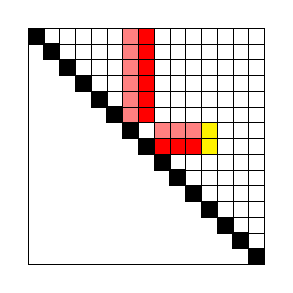
\begin{tikzpicture}[xscale=0.2,yscale=-0.2,baseline=-40]
      \fill [yellow] (12,6) -- (12,8) -- (11,8) -- (11,6) -- cycle;
      \fill [red!50] (8,6) -- (8,7) -- (11,7) -- (11,6) -- cycle;
      \fill [red!100] (8,7) -- (8,8) -- (11,8) -- (11,7) -- cycle;
      \fill [red!50] (6,0) -- (6,6) -- (7,6) -- (7,0) -- cycle;
      \fill [red!100] (7,0) -- (7,6) -- (8,6) -- (8,0) -- cycle;

      \draw (0,0) -- (15,0) -- (15,15) -- (0,15) -- cycle;
      \foreach \x in {1,2,...,14}
      {
        \draw [very thin] (\x,\x) -- (15,\x);
        \draw [very thin] (\x,0) -- (\x,\x);
      }
      \foreach \x in {0,1,...,14}
        \filldraw (\x,\x) -- (\x,\x+1) -- (\x+1,\x+1) -- (\x+1,\x) -- cycle;
    \end{tikzpicture}
    \qquad \leadsto \qquad
    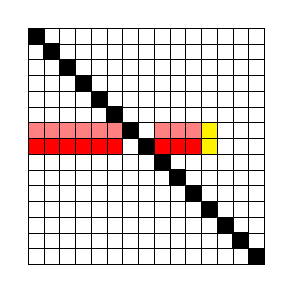
\begin{tikzpicture}[xscale=0.2,yscale=-0.2,baseline=-40]
      \fill [yellow] (12,6) -- (12,8) -- (11,8) -- (11,6) -- cycle;
      \fill [red!50] (8,6) -- (8,7) -- (11,7) -- (11,6) -- cycle;
      \fill [red!100] (8,7) -- (8,8) -- (11,8) -- (11,7) -- cycle;
      \fill [red!50] (0,6) -- (6,6) -- (6,7) -- (0,7) -- cycle;
      \fill [red!100] (0,7) -- (6,7) -- (6,8) -- (0,8) -- cycle;

      \draw (0,0) -- (15,0) -- (15,15) -- (0,15) -- cycle;
      \foreach \x in {1,2,...,14}
      {
        \draw [very thin] (0,\x) -- (15,\x);
        \draw [very thin] (\x,0) -- (\x,15);
      }
      \foreach \x in {0,1,...,14}
        \filldraw  (\x,\x) -- (\x,\x+1) -- (\x+1,\x+1) -- (\x+1,\x) -- cycle;
    \end{tikzpicture}
    \]
  \item If $a_{i, j-1} > a_{i, j}$, then there should be a division
    before $j$, i.e.\ there should be a couple in the red area for
    which the darker is strictly greater than the lighter; on the
    right, the simplification shows that the condition takes the same
    form of the previous one:
    \[
    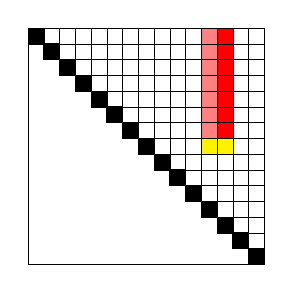
\begin{tikzpicture}[xscale=0.2,yscale=-0.2,baseline=-40]
      \fill [yellow] (13,7) -- (13,8) -- (11,8) -- (11,7) -- cycle;
      \fill [red!50] (11,0) -- (11,7) -- (12,7) -- (12,0) -- cycle;
      \fill [red!100] (12,0) -- (12,7) -- (13,7) -- (13,0) -- cycle;

      \draw (0,0) -- (15,0) -- (15,15) -- (0,15) -- cycle;
      \foreach \x in {1,2,...,14}
      {
        \draw [very thin] (\x,\x) -- (15,\x);
        \draw [very thin] (\x,0) -- (\x,\x);
      }
      \foreach \x in {0,1,...,14}
        \filldraw (\x,\x) -- (\x,\x+1) -- (\x+1,\x+1) -- (\x+1,\x) -- cycle;
    \end{tikzpicture}
    \qquad \leadsto \qquad
    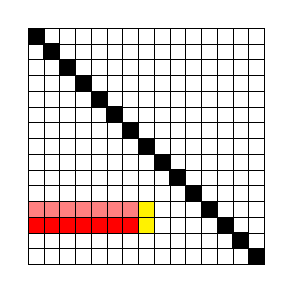
\begin{tikzpicture}[xscale=0.2,yscale=-0.2,baseline=-40]
      \fill [yellow] (7,13) -- (8,13) -- (8,11) -- (7,11) -- cycle;
      \fill [red!50] (0,11) -- (7,11) -- (7,12) -- (0,12) -- cycle;
      \fill [red!100] (0,12) -- (7,12) -- (7,13) -- (0,13) -- cycle;

      \draw (0,0) -- (15,0) -- (15,15) -- (0,15) -- cycle;
      \foreach \x in {1,2,...,14}
      {
        \draw [very thin] (0,\x) -- (15,\x);
        \draw [very thin] (\x,0) -- (\x,15);
      }
      \foreach \x in {0,1,...,14}
        \filldraw (\x,\x) -- (\x,\x+1) -- (\x+1,\x+1) -- (\x+1,\x) -- cycle;
    \end{tikzpicture}
    \]
  \end{enumerate}

  Summarizing, using the fact that the matrix $a$ is symmetric, we can
  provide the desired characterization of the stable graphs generated
  by the algorithm.
\end{proof}

\begin{definition}
  Let $G = (g, n, l, a) \in \mathcal{A}$. A piece of data $g_i$,
  $n_i$, $l_i$, or $a_{i,j}$ is called a \emph{breaking position\/} if
  it does not satisfy the four conditions of
  Lemma~\ref{lemma:char1}. 
\end{definition}

In particular, in view of the last definition, Lemma \ref{lemma:char1} translates into the following statement: \emph{A stable graph $G \in \mathcal{A}$ has a breaking position
  if and only if $G$ is not an element of $\mathcal{M}$}.

We now introduce a total order on the set $\mathcal{A}$ of graphs $G = (g,n,l,a)$. If $G$ is such a graph, let $v(G)$ be the vector obtained by
juxtaposition of the vectors $g$, $n$, $l$ and of the rows of the
upper triangular part of $a$. For example, if
\begin{align*}
  &\begin{aligned}
    G = \biggl(&g = (0,0,2,0),\\
    &\qquad \qquad n = (1,1,0,1),\\[6pt]
    &\qquad \qquad \qquad \qquad l = (0,0,0,0),\\
    &\qquad \qquad \qquad \qquad \qquad \qquad a = \psm{ 0 & 1 & 1 &
      1\\ 1 & 0 & 2 & 1\\ 1 & 2 & 0 & 0 \\ 1 & 1 & 0 & 0 }
    \biggr)\text{,}
  \end{aligned}
  && \eqqcolon &&\psm{ 0 & 0 & 2 & 0\\ 1 & 1 & 0 & 1\\ 0 & 0 & 0 & 0\\
    & 1 & 1 & 1\\ && 2 & 1\\ &&& 0 }
\end{align*}
then
\[
v(G) = (0, 0, 2, 0,\quad 1, 1, 0, 1,\quad 0, 0, 0, 0,\quad 1, 1,
1,\quad 2, 1,\quad 0)\,\text{.}
\]

\begin{definition} \label{def:order} If $G, H \in \mathcal{A}$, we
  write $G \prec H$ if and only if $v(G)$ is smaller than $v(H)$ in
  the lexicographic order.
\end{definition}

\begin{notation}
  If $\sigma \in \Sigma_K$ is a permutation and $G = (g, n, l, a)$ is
  a graph, then we can apply $\sigma$ to the entries of the data of
  $G$, obtaining an isomorphic graph. We denote this new graph by
  $\sigma G$. We denote by $\sigma_{i,j}$ the element of $\Sigma_K$ that corresponds to the transposition of $i, j \in \ubar{K}$.
\end{notation}

\begin{lemma}\label{lemma:char2}
  Let $G \in \mathcal{A}$; then $G \in \mathcal{M}$ if and only if $G$
  is minimal in the set
  \[
  \bigl\{ \sigma_{i-1,i} G \,\mid\, 1<i<K \bigr\}\text{.}
  \]
  with respect to the order given in \ref{def:order}.
\end{lemma}

\begin{proof}
  We use Lemma~\ref{lemma:char1}; in particular we prove that $G$ is
  not minimal if and only if there is a breaking position.

  Assume there are breaking positions in $G$; if the first is in $g$,
  $n$, or $l$, it is trivial to see that transposing it with the
  previous one gives a smaller graph. If breaking positions are only
  in $a$ (i.e., if $g$, $n$, and $l$ are constant), assume that
  $a_{i,j}$ is the smallest with respect to the lexicographic order on
  $(i,j)$. We deduce that for all $j^\prime < j$ not in $\{i-1,i\}$,
  we have $a_{i-1, j^\prime} = a_{i, j^\prime}$. %A priori the equality
 % sign should be a ``less or equal to'', but if the first was strictly
 % smaller than the second, then $(i,j^\prime)$ would have been a
 % smaller breaking position. 
  Let $H \coloneqq \sigma_{i-1,i} G$; the
  following pictures sum up the differences between $G$ and $H$: the
  left one represents the case $i < j$, the right one the case $i >
  j$:
  \[
  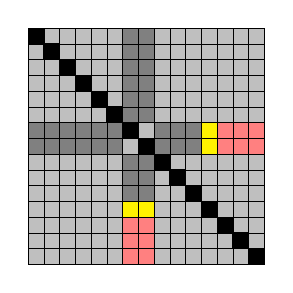
\begin{tikzpicture}[xscale=0.2,yscale=-0.2,baseline=-40]
    \fill [gray!50] (0,0) -- (15,0) -- (15,15) -- (0,15) -- cycle;
    \fill [yellow] (12,6) -- (12,8) -- (11,8) -- (11,6) -- cycle;
    \fill [yellow] (6,12) -- (8,12) -- (8,11) -- (6,11) -- cycle;
    \fill [red!50] (12,6) -- (12,8) -- (15,8) -- (15,6) -- cycle;
    \fill [red!50] (6,12) -- (8,12) -- (8,15) -- (6,15) -- cycle;
    \fill [gray] (0,6) -- (0,8) -- (11,8) -- (11,6) -- cycle;
    \fill [gray] (6,0) -- (8,0) -- (8,11) -- (6,11) -- cycle;
    \fill [gray!50] (6,6) -- (6,8) -- (8,8) -- (8,6) -- cycle;

    \draw (0,0) -- (15,0) -- (15,15) -- (0,15) -- cycle;
    \foreach \x in {1,2,...,14}
    {
      \draw [very thin] (0,\x) -- (15,\x);
      \draw [very thin] (\x,0) -- (\x,15);
    }
    \foreach \x in {0,1,...,14}
      \filldraw (\x,\x) -- (\x,\x+1) -- (\x+1,\x+1) -- (\x+1,\x) -- cycle;
  \end{tikzpicture}
  \qquad\qquad
  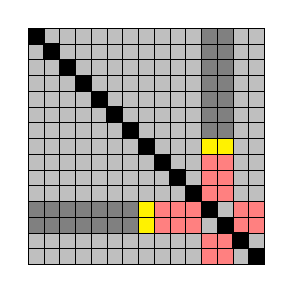
\begin{tikzpicture}[xscale=0.2,yscale=-0.2,baseline=-40]
    \fill [gray!50] (0,0) -- (15,0) -- (15,15) -- (0,15) -- cycle;
    \fill [yellow] (7,13) -- (8,13) -- (8,11) -- (7,11) -- cycle;
    \fill [yellow] (13,7) -- (13,8) -- (11,8) -- (11,7) -- cycle;
    \fill [red!50] (8,11) -- (8,13) -- (15,13) -- (15,11) -- cycle;
    \fill [red!50] (11,8) -- (13,8) -- (13,15) -- (11,15) -- cycle;
    \fill [gray] (0,11) -- (0,13) -- (7,13) -- (7,11) -- cycle;
    \fill [gray] (11,0) -- (13,0) -- (13,7) -- (11,7) -- cycle;
    \fill [gray!50] (11,11) -- (11,13) -- (13,13) -- (13,11) -- cycle;

    \draw (0,0) -- (15,0) -- (15,15) -- (0,15) -- cycle;
    \foreach \x in {1,2,...,14}
    {
      \draw [very thin] (0,\x) -- (15,\x);
      \draw [very thin] (\x,0) -- (\x,15);
    }
    \foreach \x in {0,1,...,14}
      \filldraw (\x,\x) -- (\x,\x+1) -- (\x+1,\x+1) -- (\x+1,\x) -- cycle;
  \end{tikzpicture}
  \]
  In particular:
  \begin{itemize}
  \item the yellow area is the smallest breaking position and the
    position preceding it (on its left or on the top), and the two are
    swapped in $H$;
  \item the light grey area is of course unchanged;
  \item the dark grey area is swapped, but this is unnoticeable as
    $a_{i-1,j^\prime} = a_{i,j^\prime}$;
  \item the light red area is swapped and may change the matrix.
  \end{itemize}
  So, since $a_{i-1,j} > a_{i, j}$, then $H \prec G$ and therefore $G$
  is not minimal (note that it is essential to consider only the upper
  triangular part of $a$ to define $\prec$).

  Conversely, let $i$ be such that $H \coloneqq \sigma_{i-1,i} G \prec
  G$. If the first difference between $G$ and $H$ lies in $g$, $n$, or
  $l$, then it is easy to see that the corresponding position is
  breaking. Otherwise, if the vectors $g,n,l$ are equal in $G$ and in $H$, we can see the difference between $G$ and $H$
  in the previous pictures on the matrices. Since $H \prec G$, then, going from the
  top to the diagonal and then to the right, we see that the first
  swapping that changes the matrix (that is, one that swaps different
  numbers), represented in yellow, exchanges a small number at a big
  position (with respect to the lexicographic order) with a big number
  at a small position. Hence this gives a breaking position for $G$.
\end{proof}

\begin{remark}
  Given a graph $G$, the number of graphs isomorphic to $G$ that our
  program generates is then trivially bounded by $\abs{\Sigma_K}/(K-1)
  = K\cdot (K-2)!$.
  % TODO: Give empirical estimate on the real bound (if it is linear,
  % exponential, ...)
\end{remark}

The proof of Proposition~\ref{prop:main} can now be easily deduced
arguing as in the following example.

\begin{example}
  Let $G_0 = G \in \mathcal{A}$ be the graph of the previous
  example:
  \[
  G_0 = \psm{ 0 & 0 & 2 & 0\\ 1 & 1 & 0 & 1\\ 0 & 0 & 0 & 0\\ & 1 & 1
    & 1\\ && 2 & 1\\ &&& 0 }\text{.}
  \]
  This graph is stable but not in $\mathcal{M}$ because, for example,
  $g_2 > g_3$ implies that $g_3$ is a breaking position. This is
  the smallest breaking position, thus we apply the permutation $\sigma_{2,3}$, obtaining
  the graph
  \[
  G_1 \coloneqq \sigma_{2,3} G_0 = \psm{ 0 & 0 & 0 & 2\\
    1 & 1 & 1 & 0\\ 0 & 0 & 0 & 0\\ & 1 & 1 & 1\\ && 1 & 2\\ &&& 0 }
  \prec G_0\text{.}
  \]
  Now $a_{2,3}$ is the smallest breaking position; applying
  $\sigma_{1,2}$, we obtain
  \[
  G_2 \coloneqq \sigma_{1,2} G_1 = \psm{ 0 & 0 & 0 & 2\\ 1 & 1 & 1 &
    0\\ 0 & 0 & 0 & 0\\ & 1 & 1 & 1\\ && 1 & 0\\ &&& 2 } \prec
  G_1\text{.}
  \]
  The new smallest breaking position is $a_{1,3}$, so applying the
  transposition $\sigma_{0,1}$ we have 
  \[
  G_3 \coloneqq \sigma_{0,1} G_2 = \psm{ 0 & 0 & 0 & 2\\ 1 & 1 & 1 &
    0\\ 0 & 0 & 0 & 0\\ & 1 & 1 & 0\\ && 1 & 1\\ &&& 2 } \prec
  G_2\text{.}
  \]
  The graph $G_3$ is finally in $\mathcal{M}$ and we can verify that no
  transposition can decrease it.
\end{example}

\begin{proof}[Proof of Proposition~\ref{prop:main}]
  Recall that we have to prove that for every $G \in \mathcal{A}$,
  there is a permutation $\sigma \in \Sigma_K$ such that $\sigma G \in
  \mathcal{M}$.

  So, let $G_0 = G \in \mathcal{A}$. If $G \in \mathcal{M}$, then we
  are done; otherwise, $G$ does not satisfy the condition of
  Lemma~\ref{lemma:char2}, hence there is a transposition
  $\sigma_{i-1, i}$ such that $G_1 = \sigma_{i-1,i} G_0 \prec G_0$.

  The iteration of this process comes to an end (that is, we arrive to
  a matrix in $\mathcal{M}$) since the set
  \[
  \bigl\{ \sigma G \mid \sigma \in \Sigma_K\bigr\}\text{.}\qedhere
  \]
  is finite
\end{proof}

% TODO: write a new section with some data obtained by the program,
% and consideration on running time (e.g.: running time / found
% graphs)
% \section{Performance}


\begin{thebibliography}{2}

\bibitem [BMS] {busonero}
  S.~Busonero, M.~Melo, and L.~Stoppino,
  \emph{On the complexity group of stable curves},
  \arXiv{0808.1529}.%v1

\bibitem [DM] {delignemumford}
  P.~Deligne and D.~Mumford,
  \emph{The irreducibility of the space of curves of given genus},
  Inst. Hautes \'Etudes Sci. Publ. Math. \textbf{36} (1969), 75--109.

\bibitem [F] {faber}
  C.~Faber,
  \emph{Maple program for computing Hodge integrals},
  available at \href{http://math.stanford.edu/~vakil/programs/}
  {\texttt{http://math.stanford.edu/\~{}vakil/programs/}}.

\bibitem[GK] {modularoperads}
  E.~Getzler and M.~Kapranov,
  \emph{Modular Operads},
  Compositio Math. \textbf{110} (1998), no. 1, 65--126
  [\arXiv{dg-ga/9408003}].

\bibitem [M] {nauty}
  B.~D.~McKay,
  \emph{nauty},
  available at \href{http://cs.anu.edu.au/people/bdm/nauty/}
  {\texttt{http://cs.anu.edu.au/people/bdm/nauty/}}.

\bibitem [vOV1] {opstall}
  M.~A.~van~Opstall and R.~Veliche,
  \emph{Maximally symmetric stable curves},
  Michigan Math. J. \textbf{55} (2007), no. 3, 513--534
  [\arXiv{math/0603061}].

\bibitem [vOV2] {opstall2}
  M.~A.~van~Opstall and R.~Veliche,
  \emph{Maximally symmetric stable curves II},
  \arXiv{math/0608799}.%v1

\bibitem [SY] {smith}
  G.~Smith and S.~Yang,
  \emph{HodgeIntegral. Macaulay2 package for computing Hodge Integrals},
  available by request from author \href{mailto:stpyang@math.kth.se}
  {\texttt{stpyang@math.kth.se}}.

\bibitem [Y1] {stephanie1}
  S.~Yang,
  \emph{Maple program for computing integrals on $\overline{M}_{g,n}$},
  available by request from author \href{mailto:stpyang@math.kth.se}
  {\texttt{stpyang@math.kth.se}}.

\bibitem [Y2] {stephanie2}
  S.~Yang,
  \emph{Calculating intersection numbers on moduli spaces of pointed curves},
  \arXiv{0808.1974}.%v2

\end{thebibliography}
\end{document}
